%<dscrpt>Fichier de déclarations Latex à inclure au début d'un élément de cours.</dscrpt>

\documentclass[a4paper]{article}
\usepackage[hmargin={1.8cm,1.8cm},vmargin={2.4cm,2.4cm},headheight=13.1pt]{geometry}

%includeheadfoot,scale=1.1,centering,hoffset=-0.5cm,
\usepackage[pdftex]{graphicx,color}
\usepackage[french]{babel}
%\selectlanguage{french}
\addto\captionsfrench{
  \def\contentsname{Plan}
}
\usepackage{fancyhdr}
\usepackage{floatflt}
\usepackage{amsmath}
\usepackage{amssymb}
\usepackage{amsthm}
\usepackage{stmaryrd}
%\usepackage{ucs}
\usepackage[utf8]{inputenc}
%\usepackage[latin1]{inputenc}
\usepackage[T1]{fontenc}


\usepackage{titletoc}
%\contentsmargin{2.55em}
\dottedcontents{section}[2.5em]{}{1.8em}{1pc}
\dottedcontents{subsection}[3.5em]{}{1.2em}{1pc}
\dottedcontents{subsubsection}[5em]{}{1em}{1pc}

\usepackage[pdftex,colorlinks={true},urlcolor={blue},pdfauthor={remy Nicolai},bookmarks={true}]{hyperref}
\usepackage{makeidx}

\usepackage{multicol}
\usepackage{multirow}
\usepackage{wrapfig}
\usepackage{array}
\usepackage{subfig}


%\usepackage{tikz}
%\usetikzlibrary{calc, shapes, backgrounds}
%pour la présentation du pseudo-code
% !!!!!!!!!!!!!!      le package n'est pas présent sur le serveur sous fedora 16 !!!!!!!!!!!!!!!!!!!!!!!!
%\usepackage[french,ruled,vlined]{algorithm2e}

%pr{\'e}sentation du compteur de niveau 2 dans les listes
\makeatletter
\renewcommand{\labelenumii}{\theenumii.}
\renewcommand{\thesection}{\Roman{section}.}
\renewcommand{\thesubsection}{\arabic{subsection}.}
\renewcommand{\thesubsubsection}{\arabic{subsubsection}.}
\makeatother


%dimension des pages, en-t{\^e}te et bas de page
%\pdfpagewidth=20cm
%\pdfpageheight=14cm
%   \setlength{\oddsidemargin}{-2cm}
%   \setlength{\voffset}{-1.5cm}
%   \setlength{\textheight}{12cm}
%   \setlength{\textwidth}{25.2cm}
   \columnsep=1cm
   \columnseprule=0.5pt

%En tete et pied de page
\pagestyle{fancy}
\lhead{MPSI-\'Eléments de cours}
\rhead{\today}
%\rhead{25/11/05}
\lfoot{\tiny{Cette création est mise à disposition selon le Contrat\\ Paternité-Pas d'utilisations commerciale-Partage des Conditions Initiales à l'Identique 2.0 France\\ disponible en ligne http://creativecommons.org/licenses/by-nc-sa/2.0/fr/
} }
\rfoot{\tiny{Rémy Nicolai \jobname}}


\newcommand{\baseurl}{http://back.maquisdoc.net/data/cours\_nicolair/}
\newcommand{\urlexo}{http://back.maquisdoc.net/data/exos_nicolair/}
\newcommand{\urlcours}{https://maquisdoc-math.fra1.digitaloceanspaces.com/}

\newcommand{\N}{\mathbb{N}}
\newcommand{\Z}{\mathbb{Z}}
\newcommand{\C}{\mathbb{C}}
\newcommand{\R}{\mathbb{R}}
\newcommand{\D}{\mathbb{D}}
\newcommand{\K}{\mathbf{K}}
\newcommand{\Q}{\mathbb{Q}}
\newcommand{\F}{\mathbf{F}}
\newcommand{\U}{\mathbb{U}}
\newcommand{\p}{\mathbb{P}}


\newcommand{\card}{\mathop{\mathrm{Card}}}
\newcommand{\Id}{\mathop{\mathrm{Id}}}
\newcommand{\Ker}{\mathop{\mathrm{Ker}}}
\newcommand{\Vect}{\mathop{\mathrm{Vect}}}
\newcommand{\cotg}{\mathop{\mathrm{cotan}}}
\newcommand{\sh}{\mathop{\mathrm{sh}}}
\newcommand{\ch}{\mathop{\mathrm{ch}}}
\newcommand{\argsh}{\mathop{\mathrm{argsh}}}
\newcommand{\argch}{\mathop{\mathrm{argch}}}
\newcommand{\tr}{\mathop{\mathrm{tr}}}
\newcommand{\rg}{\mathop{\mathrm{rg}}}
\newcommand{\rang}{\mathop{\mathrm{rg}}}
\newcommand{\Mat}{\mathop{\mathrm{Mat}}}
\newcommand{\MatB}[2]{\mathop{\mathrm{Mat}}_{\mathcal{#1}}\left( #2\right) }
\newcommand{\MatBB}[3]{\mathop{\mathrm{Mat}}_{\mathcal{#1} \mathcal{#2}}\left( #3\right) }
\renewcommand{\Re}{\mathop{\mathrm{Re}}}
\renewcommand{\Im}{\mathop{\mathrm{Im}}}
\renewcommand{\th}{\mathop{\mathrm{th}}}
\newcommand{\repere}{$(O,\overrightarrow{i},\overrightarrow{j},\overrightarrow{k})$}
\newcommand{\cov}{\mathop{\mathrm{Cov}}}

\newcommand{\absolue}[1]{\left| #1 \right|}
\newcommand{\fonc}[5]{#1 : \begin{cases}#2 \rightarrow #3 \\ #4 \mapsto #5 \end{cases}}
\newcommand{\depar}[2]{\dfrac{\partial #1}{\partial #2}}
\newcommand{\norme}[1]{\left\| #1 \right\|}
\newcommand{\se}{\geq}
\newcommand{\ie}{\leq}
\newcommand{\trans}{\mathstrut^t\!}
\newcommand{\val}{\mathop{\mathrm{val}}}
\newcommand{\grad}{\mathop{\overrightarrow{\mathrm{grad}}}}

\newtheorem*{thm}{Théorème}
\newtheorem{thmn}{Théorème}
\newtheorem*{prop}{Proposition}
\newtheorem{propn}{Proposition}
\newtheorem*{pa}{Présentation axiomatique}
\newtheorem*{propdef}{Proposition - Définition}
\newtheorem*{lem}{Lemme}
\newtheorem{lemn}{Lemme}

\theoremstyle{definition}
\newtheorem*{defi}{Définition}
\newtheorem*{nota}{Notation}
\newtheorem*{exple}{Exemple}
\newtheorem*{exples}{Exemples}


\newenvironment{demo}{\renewcommand{\proofname}{Preuve}\begin{proof}}{\end{proof}}
%\renewcommand{\proofname}{Preuve} doit etre après le begin{document} pour fonctionner

\theoremstyle{remark}
\newtheorem*{rem}{Remarque}
\newtheorem*{rems}{Remarques}

\renewcommand{\indexspace}{}
\renewenvironment{theindex}
  {\section*{Index} %\addcontentsline{toc}{section}{\protect\numberline{0.}{Index}}
   \begin{multicols}{2}
    \begin{itemize}}
  {\end{itemize} \end{multicols}}


%pour annuler les commandes beamer
\renewenvironment{frame}{}{}
\newcommand{\frametitle}[1]{}
\newcommand{\framesubtitle}[1]{}

\newcommand{\debutcours}[2]{
  \chead{#1}
  \begin{center}
     \begin{huge}\textbf{#1}\end{huge}
     \begin{Large}\begin{center}Rédaction incomplète. Version #2\end{center}\end{Large}
  \end{center}
  %\section*{Plan et Index}
  %\begin{frame}  commande beamer
  \tableofcontents
  %\end{frame}   commande beamer
  \printindex
}


\makeindex
\begin{document}
\noindent

\debutcours{Convexité}{beta}

\section{Parties convexes}
Dans cette section, on se place dans un $\R$ espace vectoriel $E$ dont les éléments seront considérés comme des \emph{points} ou des \emph{vecteurs}.
\begin{defi}[Segment]
 Soit $x$ et $y$ deux points de $E$, le segment (noté $[x,y]$) d'extrémités $x$ et $y$ est défini par :
\begin{displaymath}
 [x,y] = \left\lbrace \lambda x + (1-\lambda) y , \lambda \in [0,1]\right\rbrace 
\end{displaymath}
\end{defi}
\begin{rems}
 \begin{itemize}
 \item On peut adopter un point  de vue \emph{barycentrique}. Le point $\lambda x + (1-\lambda) y$ est le barycentre des points $x$ et $y$ affectés des masses $\lambda$ et $1-\lambda$. Le segment $[x,y]$ est donc formé par l'ensemble des barycentres de $x$ et $y$ affectés de coefficients positifs et de somme 1.
\item On peut aussi adopter un point de vue \emph{cinématique}. La fonction $t \rightarrow x +t (y-x)$ pour $t\in[0,1]$ représente le mouvement d'un point qui part de $x$ et va vers $y$ à la vitesse constante $y-x$. Le segment $[x,y]$ est alors la \emph{trajectoire} du mouvement.
\item On passe d'un point de vue à l'autre par $\lambda = 1-t$.
\item Un sous-espace affine de $E$ est une partie convexe.
\end{itemize}
\end{rems}
\begin{figure}[h]
  \begin{minipage}{.4\linewidth}
     \centering
     \input{C2071_1.pdf_t} 
     \caption{Partie convexe}
  \end{minipage}
  \hfill
  \begin{minipage}{.4\linewidth}
     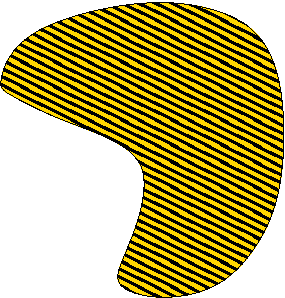
\includegraphics{C2071_2.pdf}
     % C2071_1.pdf: 139x114 pixel, 72dpi, 4.90x4.02 cm, bb=0 0 139 114
     \caption{Partie non convexe}
   \end{minipage}
\end{figure}
\index{partie convexe}
\begin{defi}[Partie convexe]
Une partie $A$ d'un $\R$ espace vectoriel $E$ est convexe lorsque, pour tous les points $x$ et $y$ de $A$, le segment $[x,y]$ est inclus dans $A$. 
\end{defi}
\index{associativité des barycentres}
\begin{prop}[associativité des barycentres]
 à rédiger
\end{prop}
\begin{demo}
 à rédiger
\end{demo}

\index{stabilité par barycentration positive}
\begin{prop}
 Une partie $A$ de $E$ est convexe si et seulement si pour tout entier $n\geq2$, pour toute famille $(x_1,\cdots,x_n)$ de points de $A$, pour toute famille $(\lambda_1,\cdots,\lambda_n)$ de réels positifs tels que $\lambda_1 + \cdots +\lambda_n =1$ on a :
\begin{displaymath}
 \lambda_1 x_1+ \cdots +\lambda_n x_n \in A
\end{displaymath}
\end{prop}
\begin{demo}
 \begin{itemize}
 \item Lorsque la propriété est vérifiée pour tous les $n$, elle l'est en particulier pour $n=2$ ce qui donne exactement la définition de la convexité.
 \item Dans l'autre sens, le passage de $2$ à $n$ se fait par récurrence. Il s'agit essentiellement de \emph{l'associativité des barycentres}. Tout repose sur la relation :
\begin{displaymath}
 \lambda_1 x_1+ \cdots +\lambda_n x_n =
  \lambda_1 x_1 +(1-\lambda_1)\left(\dfrac{\lambda_2}{\lambda_2 + \cdots + \lambda_n}x_2 + \cdots + \dfrac{\lambda_n}{\lambda_2 + \cdots + \lambda_n}x_n \right) 
\end{displaymath}
valable car $1-\lambda_1 = \lambda_2 + \cdots + \lambda_n$.
\end{itemize}

\end{demo}

\begin{prop}
 Une intersection de parties convexes est convexe.
\end{prop}
\begin{demo}
 Immédiat avec les définitions.
\end{demo}

\begin{prop}
 Les partie convexes de $\R$ (considéré comme un $\R$-espace vectoriel) sont les intervalles.
\end{prop}
\begin{demo}
 Ceci résulte de la propriété de la borne supérieure. La démonstration de ce résultat figure dans la section \href{\baseurl C2192.pdf}{Axiomatique du corps des réels}  
\end{demo}

\begin{prop}
 L'image d'une partie convexe par une application affine est convexe.
\end{prop}
\begin{demo}
 Immédiat avec les définitions.
\end{demo}
\begin{exples}
 Un demi-espace est convexe. Un sous-espace affine est convexe.
\end{exples}

\section{Fonctions convexes}
Dans toute cette partie $f$ désigne une fonction à valeurs réelles et définie dans un intervalle $I$ non réduit à un point.
\subsection{Définition}
\begin{figure}[ht]
 \centering
 \input{C2071_3.pdf_t}
\caption{Définition $\Gamma_f^+$ et $\Gamma_f^-$}
\end{figure}
\index{fonction convexe}
\begin{defi}[Fonction convexe]
 Soit $I$ un intervalle de $\R$ non réduit à un point. Une $f$ une fonction à valeurs réelles définie dans $I$ est convexe lorsque :
\begin{displaymath}
 \forall (x,y)\in I^2 , \forall \lambda \in [0,1]\; :\; f(\lambda_1 x+\lambda_2 y)\leq \lambda_1 f(x)+\lambda_2 f(y)
\end{displaymath}
\end{defi}
\begin{rem}
 La définition précédente peut aussi s'écrire (en adoptant le point de vue barycentrique)
\begin{displaymath}
 \forall (x,y)\in I^2 , \forall (\lambda_1,\lambda_2) \in [0,1]^2 \text{ tels que } \lambda_1+\lambda_2=1\; :\; f((1-\lambda)x+\lambda y)\leq (1-\lambda)f(x)+\lambda f(y)
\end{displaymath}
ou encore (en adoptant le point de vue cinématique)
\begin{displaymath}
 \forall (x,y)\in I^2 , \forall \lambda \in [0,1] \text{ tels que } \; :\; f(x+\lambda (y-x))\leq f(x)+\lambda (f(y)-f(x)
\end{displaymath}
\end{rem}

\index{fonction concave}
\begin{defi}[Fonction concave]
Une fonction $f$ est concave si et seulement si $-f$ est convexe.
\end{defi}
\begin{prop}
  Une fonction $f$ est convexe si et seulement si $\Gamma_f^+$ est une partie convexe de $\R^2$ et $f$ est concave si et seulement si $\Gamma_f^-$ est une partie convexe de $\R^2$. Les parties $\Gamma_f^+$ et $\Gamma_f^-$ étant définies par :
\begin{displaymath}
 \Gamma_f^- = \left\lbrace (x,y)\in I\times \R \text{ tq } y\geq f(x) \right\rbrace, \quad
 \Gamma_f^+ = \left\lbrace (x,y)\in I\times \R \text{ tq } y\leq f(x) \right\rbrace
\end{displaymath}
\end{prop}
\begin{nota}
 On désigne par $M_x$ le point de coordonnées $(x,f(x))$ du graphe de $f$. un segment $[M_x,M_y]$ dont les extrémités sont deux points du graphe est une \emph{corde} du graphe.
\end{nota}
\begin{prop}
 Une fonction est convexe si et seulement si son graphe est \emph{au dessous} de ses cordes.
\end{prop}
\begin{figure}[ht]
 \centering
 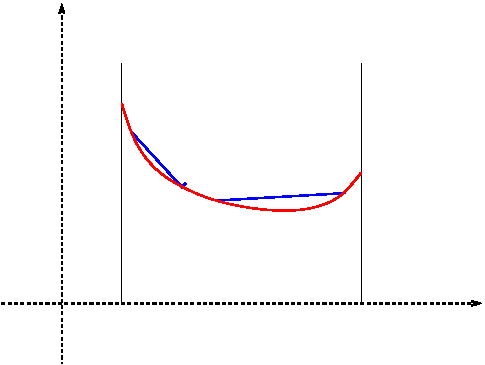
\includegraphics{C2071_4.pdf}
 % C2070_4.pdf: 1179666x1179666 pixel, 0dpi, infxinf cm, bb=
 \caption{Le graphe d'une fonction convexe est au dessous de ses cordes}
\end{figure}
\index{inégalité de convexité}
\begin{prop}[Inégalité de convexité]
 Une fonction $f$ est convexe si et seulement si pour tout entier $n\geq2$, pour toute famille $(x_1,\cdots,x_n)$ d'éléments de $I$, pour toute famille $(\lambda_1,\cdots,\lambda_n)$ de réels positifs tels que $\lambda_1 + \cdots +\lambda_n =1$ on a :
\begin{displaymath}
 f(\lambda_1 x_1+ \cdots +\lambda_n x_n) \leq \lambda_1f(x_1)+\cdots +\lambda_n f(x_n)
\end{displaymath}
\end{prop}
\begin{rem}
 Cette inégalité est aussi appelée \emph{inégalité de Jensen discrète}. \index{inégalité de Jensen discrète}
\end{rem}

\subsection{Caractérisations}
Dans la pratique les fonctions dont on a à étudier la convexité sont $\mathcal C ^2$ et on exploite cette propriété avec l'inégalité de convexité.
\subsubsection{Croissance des taux d'accroissements}
\begin{nota}[Taux d'accroissement]
 Pour tout $x\in I$, on désigne par $\Phi_x$ la fonction définie dans $I\setminus\{x\}$ par :
\begin{displaymath}
 \Phi_x(t)= \dfrac{f(t)-f(x)}{t-x} = \dfrac{f(x)-f(t)}{x-t}
\end{displaymath}
\end{nota}
\hyperdef{prop}{croi_taux}{}
\begin{prop}
 Une fonction $f$ est croissante si et seulement si toutes les fonctions $\Phi_x$ sont croissantes (pour tous les $x\in I$).
\end{prop}
\begin{rem}
 Il s'agit de la croissance dans $I\setminus\{x\}$ tout entier et non des croissances indépendantes des restrictions aux deux intervalles constituant $I\setminus\{x\}$.
\begin{displaymath}
 \forall (u,v)\in (I\setminus\{x\})^2 : u\leq v \Rightarrow \Phi_x(u) \leq \Phi_x(v)
\end{displaymath}
\end{rem}
\begin{demo}
 \begin{description}
   \item[Convexité entraîne croissance des taux] On suppose la fonction convexe. On considère un $x$ quelconque dans $I$, on veut montrer la croissance de $\Phi_x$. Soit $u$ et $v$ dans $I\setminus\{x\}$ avec $u<v$. Plusieurs cas sont possibles mais il y a toujours un point dans l'intervalle formé par les deux autres. On peut former une inégalité de convexité attachée à cette configuration (bien prendre garde aux signes des coefficients).
\begin{multline*}
 x<u<v \Rightarrow u=x+\dfrac{u-x}{v-x}(v-x) \Rightarrow
 f(u)\leq f(x)+\dfrac{u-x}{v-x}(f(v)-f(x)) \Rightarrow \Phi_x(u)\leq \Phi_x(v)
\end{multline*}
\begin{multline*}
 u<x<v \Rightarrow x=u+\dfrac{x-u}{v-u}(v-u) \Rightarrow
 f(x)\leq f(u)+\dfrac{x-u}{v-u}\underbrace{(f(v)-f(u))}_{f(v)-f(x)+f(x)-f(u)}\\
 \Rightarrow  \left(1-\dfrac{x-u}{v-u} \right)(f(x)-f(u))\leq \dfrac{x-u}{v-u}(f(v)-f(x)) \Rightarrow \Phi_x(u)\leq \Phi_x(v)
\end{multline*}
\begin{multline*}
 u<v<x \Rightarrow v=u+\dfrac{v-u}{x-u}(x-u) \Rightarrow
 f(v)\leq f(u)+\dfrac{v-u}{x-u}(f(x)-f(u)) \\ 
\Rightarrow f(v)-f(x)\leq \left( -1+\dfrac{v-u}{x-u}\right) (f(x)-f(u)) \\
\Rightarrow f(v)-f(x)\leq -\dfrac{x-v}{x-u} (f(x)-f(u))
\Rightarrow \Phi_x(u)\leq \Phi_x(v)
\end{multline*}

   \item[Croissance des taux entraîne convexité] Soit $x$ et $y$ dans $I$ (on peut supposer $x<y$) et $\lambda\in]0,1[$. On pose $u_\lambda = x +\lambda (x-y)$. On vérifie alors facilement que 
\begin{displaymath}
\Phi_{u_\lambda}(x)\leq \Phi_{u_\lambda}(y) \Rightarrow f(x) \leq \lambda (f(y)-f(x)) 
\end{displaymath}
 \end{description}
\end{demo}

La proposition suivante n'est pas au programme de MPSI mais se déduit facilement de la croissance des taux.
\begin{prop}
 Soit $f$ une fonction convexe dans un intervalle $I$ et $\mathring{I}$ l'intervalle privé de ses extrémités.
\begin{itemize}
 \item $f$ est continue dans $\mathring{I}$
 \item $f$ est dérivable à droite (dérivée $f_d^\prime$) et à gauche (dérivée $f_g^\prime$) dans $\mathring{I}$
 \item $f_d^\prime$ et $f_g^\prime$ sont croissantes et vérifient
\begin{displaymath}
 \forall (x,y)\in \mathring{I}^2 \text{ tels que } x<y \;:\;
f_g^\prime(x)\leq f_d^\prime(x) \leq \dfrac{f(y)-f(x)}{y-x} \leq f_g^\prime(y) \leq f_d^\prime(y)
\end{displaymath}

\end{itemize}

\end{prop}

\subsubsection{Cas des fonctions dérivables}
Dans cette partie, $f$ est une fonction continue et dérivable dans $I$.
\begin{figure}[ht]
 \centering
 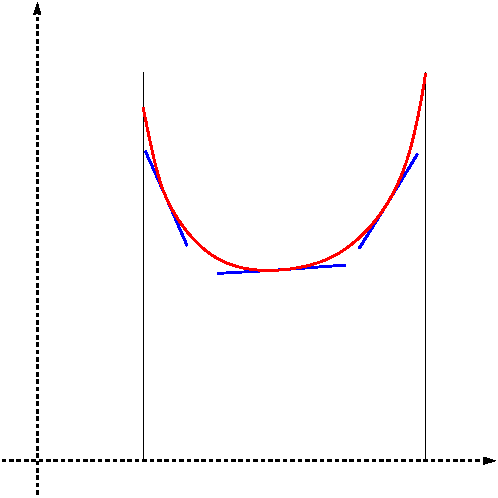
\includegraphics{C2071_5.pdf}
 % C2070_4.pdf: 1179666x1179666 pixel, 0dpi, infxinf cm, bb=e
 \caption{Le graphe d'une fonction convexe est au dessus de ses tangentes}
\end{figure}
\begin{prop}
 Les trois propriétés suivantes sont équivalentes
\begin{itemize}
 \item $f$ est convexe 
 \item $f^\prime$ est croissante
 \item le graphe de $f$ est au dessus de ses tangentes
\end{itemize}
\end{prop}
\begin{rem}
 Dans le cas où la fonction est deux fois dérivable dans $I$, elle est convexe si et seulement si la dérivée seconde ne prend que des valeurs positives.
\end{rem}
\begin{demo} Ici $f$ est dérivable, on utilisera la caractérisation de la convexité par la croissance des taux. Avant de prouver les implications, remarquons que le graphe de $f$ est au dessus de ses tangentes se traduit par :
\begin{displaymath}
 \forall (x,y)\in I^2 \;:\; f(y)\geq f(x) + f'(x)(y-x) 
\end{displaymath}

 \begin{description}
 \item [Convexité entraîne dérivée croissante.] Soit $x$ et $y$ deux éléments dans $I$ tels que $x<y$. Pour tout $u$ et $v$ dans $]x,y[$ tels que $u<v$, on peut écrire :
\begin{displaymath}
 \Phi_u(x)\leq\Phi_u(v)=\Phi_v(u)\leq\Phi_v(y)
\end{displaymath}
 Par passage à la limite dans l'inégalité quand $u\rightarrow x$ dans $]x,y[$, on obtient :
\begin{displaymath}
 \forall v\in ]x,y[\;:\; f'(x)\leq \Phi_v(y)
\end{displaymath}
 Par passage à la limite dans l'inégalité quand $v\rightarrow y$ dans $]x,y[$, on obtient :
\begin{displaymath}
  f'(x)\leq f'(y)
\end{displaymath}

 \item [Dérivée croissante entraîne graphe au dessus de ses tangentes.] 
 Soit $x$ et $y$ dans $I$ avec $x\neq y$. D'après l'inégalité des accroissements finis entre $x$ et $y$ puis en exploitant la croissance de $f'$
\begin{displaymath}
 f'(\min(x,y))\leq \dfrac{f(y)-f(x)}{y-x}\leq f'(\max(x,y)).
\end{displaymath}
Si $x<y$ alors $y-x>0$ et on utilise l'inégalité de gauche. Si $y<x$ alors $y-x<0$ et on utilise l'inégalité de droite. Dans les deux cas on aboutit à :
\begin{displaymath}
 f(y)\geq f(x) + f'(x)(y-x) 
\end{displaymath}

 \item [Graphe au dessus de ses tangentes entraîne convexité.] Soit $y$ un élément quelconque de $I$. On veut montrer que $\Phi_y$ est croissante. Le point important est que la dérivabilité de $f$ entraîne la possibilité de prolonger $\Phi_y$ par continuité en $y$. On pose donc $\Phi_y(y)=f'(y)$. En revanche $\Phi_y$ n'est dérivable que dans $I\setminus\{y\}$ avec :
\begin{displaymath}
 \forall x\in I\setminus\{y\}\;:\; \Phi_y ^\prime (x)=\dfrac{1}{(x-y)^2}\left(f'(x)(x-y)- f(x)+f(y)\right) \geq 0
\end{displaymath}
car le graphe est au dessus de ses tangentes. La croissance dans chaque intervalle de dérivabilité et la continuité dans l'intervalle complet entraîne la croissance des $\Phi_y$ donc la convexité de $f$.
\end{description}
\end{demo}
\begin{exples}
 \begin{itemize}
 \item Pour $x>0$ : $\ln''(x)=-\frac{1}{x^2}$ donc $\ln$ est concave et $-\ln$ est convexe.\newline
\'Ecrire l'inégalité de convexité avec $n$ réels $x_1,\cdots,x_n$ strictement positifs et tous les coefficients égaux à $\frac{1}{n}$ conduit à la comparaison entre les moyennes arithmétique (notée $a$), géométrique (notée $g$) et harmonique (notée $h$).
\index{moyenne arithmétique}\index{moyenne géométrique}\index{moyenne harmonique}
\begin{displaymath}
 -\ln\left(\dfrac{1}{n}x_1+\cdots+ \dfrac{1}{n}x_n \right) \leq -\dfrac{1}{n}\ln(x_1)-\cdots -\dfrac{1}{n}\ln(x_n)
\end{displaymath}
En changeant les signes et en composant par l'exponentielle qui est croissante, on obtient
\begin{align*}
 (x_1.\cdots x_n)^{\frac{1}{n}} &\leq \dfrac{x_1+\cdots + x_n}{n}\\
 g &\leq a
\end{align*}
avec 
\begin{align*}
 a = \dfrac{x_1+\cdots+x_n}{n} & & g = \left(x_1\cdots x_n \right)^{\frac{1}{n}} & & h = \dfrac{n}{\dfrac{1}{x_1}+\cdots +\dfrac{1}{x_n}} 
\end{align*}
Si on pose $y_i=\frac{1}{x_i}$ dans l'inégalité de convexité, on obtient
\begin{displaymath}
 -\ln\left(\dfrac{1}{n}\dfrac{1}{y_1}+\cdots+ \dfrac{1}{n}\dfrac{1}{y_n} \right) \leq +\dfrac{1}{n}\ln(y_1)+\cdots +\dfrac{1}{n}\ln(y_n)
\end{displaymath}
En composant par l'exponentielle qui est croissante, on obtient la comparaison entre les moyennes des $y_i$ mais tous ces nombres sont quelconques. Donc :
\begin{displaymath}
 h \leq g
\end{displaymath}


\item Dans $[0,\frac{\pi}{2}]$, la fonction $-\sin$ est convexe. En écrivant les propriétés de position du graphe par rapport à une corde et une tangente, on obtient :
\begin{displaymath}
 \dfrac{2}{\pi}x\leq \sin x\leq x
\end{displaymath}
\end{itemize}
\end{exples}

\end{document}
